\documentclass[acronym,symbols]{fei}
\usepackage[utf8]{inputenc}

\usepackage{subcaption} 
\usepackage{graphicx}
\usepackage{amsmath} % for the equation* environment
\usepackage{float}
\usepackage[portuguese]{algorithm2e}
\usepackage{biblatex}
\usepackage{listings}
\usepackage{chngcntr} 
\usepackage{appendix}
\counterwithout{footnote}{chapter}
\usepackage{siunitx}
\sisetup{output-exponent-marker=\ensuremath{\mathrm{e}}}
\renewcommand{\cftfigurepresnum}{Figura }
\setlength{\cftfigurenumwidth}{5.7em}
\usepackage{titling}

\title{Avaliação do condicionamento do ar da frota J ou H do metro de São Paulo}
\author{Ana Sung Marques \\Felipe Estevão Coquito de Mello\\  Gabriel de Souza Simonetti  \\ Gabriel Mola da Silva \\ Netuno Trindade Torrente Rovaroto \\ Victor Salzo Lopes  \\ Vitoria Fedatto Stefaneli}
\cidade{São Bernardo do Campo}
\instituicao{Centro Universitário FEI}

\addbibresource{Referencias.bib}
%\bibliographystyle{plain}
\bibliography{Referencias}
\graphicspath{ {Imagens/}, {Tabelas/}}

\begin{document}
\maketitle

\begin{folhaderosto}
	Trabalho de Conclusão de Curso apresentado ao Centro Universitário FEI, como parte dos requisitos necessários para obtenção do título de Bacharel em Engenharia Mecânica. Orientado pelo Prof. Dr. Cyro Albuquerque Neto.
\end{folhaderosto}

\begin{agradecimentos}

\end{agradecimentos}

\begin{resumo}
O Metrô de São Paulo é a maior rede de transporte público do país, com cerca de um bilhão de passageiros transportados anualmente. No entanto, ainda enfrenta um grande problema: o conforto térmico dentro dos carros. O serviço possui canais de reclamações e, segundo informações fornecidas via SMS e redes sociais, no ano de 2023, o maior volume de reclamações foi em relação à ventilação e ar-condicionado. Visando melhorar o conforto térmico e a diminuição das reclamações, será realizado um estudo por meio de uma parceria do Metrô São Paulo com o Centro Universitário FEI. Dessa forma, o objetivo principal do trabalho será analisar as condições atuais de conforto térmico para os passageiros do Metrô, buscando, assim, possíveis soluções para o sistema já existente. Para atingir o objetivo proposto, torna-se necessária a utilização de sensores para medir determinadas propriedades do ar, correlacionando-as com reclamações dos passageiros e a norma técnica vigente. Nesse contexto, o trabalho tem como principal meta o desenvolvimento de uma placa de sensoriamento que permita analisar as propriedades do ar, tais como: temperatura, umidade, concentração de $CO_2$ e produção de contaminantes. Posteriormente, os sensores deverão ser posicionados dentro dos carros do Metrô, permitindo a coleta dos dados e comparando-os com a norma utilizada atualmente, no caso, a $NBR-16.401-2$. Em uma etapa mais avançada, o sistema será estudado mediante simulações de elementos finitos no $software$ $Ansys$, visando observar se o posicionamento dos dutos de insuflamento e exaustão são realmente eficientes. 

\palavraschave{Metrô. Condicionamento de ar. Transporte público.}

\end{resumo}

%\begin{abstract}

    %\keywords{}    

%\end{abstract}

\listoffigures
%\listoftables
\tableofcontents

\chapter{Introdução}

A Companhia Metropolitana de São Paulo – Metrô foi constituída no dia 24 de abril de 1968, e é considerada um incrível marco na engenharia e planejamento urbano da cidade de São Paulo. Ela surgiu como uma solução vital para o transporte das inúmeras pessoas na região metropolitana de São Paulo, e com o rápido crescimento populacional, este meio de transporte é cada vez mais essencial na vida dos paulistas. 

No entanto, por mais que o metrô seja uma excelente proposta para mitigar os problemas de tráfego e transporte enfrentados na metrópole, ele enfrenta diversos desafios, incluindo a lotação em horários de pico, com milhões de pessoas fazendo uso deste meio de transporte todos os dias, além da necessidade de melhoria na manutenção de infraestrutura.

Com essa quantidade enorme de pessoas utilizando este meio de transporte, um dos maiores desafios para os responsáveis é fornecer ambientes internos agradáveis e seguros. Isso destaca ainda mais a necessidade de estudar a respeito do conforto térmico e a qualidade do ar dentro dos vagões, desenvolvendo e propondo uma solução para esta problemática.

\section{Motivação}

A cidade de São Paulo é a maior cidade do Brasil, com mais de 11 milhões de habitantes \cite{IBGE} e com seu crescimento acelerado e sem planejamento traz discussões a respeito de soluções para a mobilidade urbana na cidade. Portanto, cria-se a necessidade de incentivar a utilização de transportes coletivos. Desse modo, proporcionar uma experiência agradável nos transportes públicos auxilia no desenvolvimento positivo da mobilidade urbana de São Paulo.

O meio de transporte mais amplamente utilizado na grande São Paulo é o Metrô. E uma das maiores problemáticas atribuídas ao Metrô de São Paulo reside na qualidade do ar e na temperatura interna nos vagões \cite{MetroSP}. 
Essa questão ressalta a urgência de um estudo que proponha a solução para os problemas de ventilação dentro dos carros das frotas do Metrô.

\section{Objetivo geral}


O objetivo deste trabalho é realizar um sensoriamento do interior e exterior dos carros do Metrô, medindo parâmetros que influenciem no condicionamento do ar e conforto térmico dos passageiros. Pretende-se correlacionar os dados obtidos com as reclamações recebidas via SMS pelo Metrô, entendendo melhor a percepção dos passageiros em relação à qualidade do ar nos vagões. Além disso, avaliar sua conformidade com os padrões estipulados em normas e sugerir possíveis melhorias e oportunidades para estudos futuros.


\section{Objetivos específicos}


\begin{itemize}
    \item[1 -]Reunião com a equipe do Metrô de São Paulo para aquisição dos dados relevantes para o trabalho, tais como: reclamações via SMS, estatísticas a respeito do Metrô, desenhos do equipamento de HVAC, etc; 
    \item[2 -]Desenvolvimento das placas de sensoriamento com base em $Arduino$, posicionadas em locais estratégicos do vagão, visando medir propriedades a serem observadas, como: temperatura, umidade, concentração de gás carbônico, particulados e pressão barométrica;
    \item[3 -]Visita técnica no Metrô de São Paulo, buscando estudar o melhor posicionamento dos sensores mencionados, evitando deste forma desvios na aquisição dos dados;
    \item[4 -]Coleta, interpretação e analise detalhada dos dados dos sensores;
    \item[5 -]Estudo realizado através do $Software$ $Ansys$, visando otimizar o posicionamento dos dutos de insuflamento e exaustão;
    \item[6 -]Possíveis sugestões de melhoria para o sistema de ventilação.
\end{itemize}

\chapter{Referências Bibliográficas}

Para se conseguir um ambiente termicamente agradável é necessário avaliar alguns parâmetros e condições do ar. Para isso, leva-se em consideração a ventilação, as trocas de calor com o ambiente, as produções de energia térmica, os contaminantes e taxas metabólicas. Portanto, aplica-se balanços de energia para se calcular o conforto térmico no espaço.

\section{Conforto térmico}

Conforto térmico é a condição mental que expressa satisfação com o ambiente térmico e é uma avaliação subjetiva \cite{ASHRAE2009}.

Segundo \textcite{konstantinov2015numerical}, o conforto térmico dos passageiros se tornou um critério de design importante para os fabricantes de trens. Isso porque, apesar das sensações individuais serem bem diferentes umas das outras, elas dependem do fluxo de ar, da distribuição de temperatura dentro do ambiente e da radiação de calor na cabine. É por essa questão que o estudo de conforto térmico foca na ventilação e qualidade do ar.

Com base em estudo realizado por \textcite{casellisimulaccao}, um vagão de trem se encontra em diferentes situações em relação à troca de calor do ambiente, portanto, existe um índice que representa um nível aceitável de conforto térmico para as pessoas. Esse índice depende de alguns parâmetros físicos, processos fisiológicos, psicológicos e culturais.

Em pesquisas anteriores de \textcite{TCCThomas}, tem-se uma análise comparativa do conforto térmico entre as linhas vermelha e azul do metrô de São Paulo, na qual sensores de temperatura e umidade foram dispostos no interior de um carro da linha vermelha durante o trajeto de ida e volta usualmente percorrido pelo mesmo. Dessa maneira, a coleta de dados ocorreu das 16h08 às 17h29, e foi comparada com simulações realizadas no software $Ansys$ $Fluent$, além de avaliar em relação às normas existentes (\cite{en200614750} e \cite{handbook2006american}). Deste modo, foi notada uma influência do fluxo de passageiros na temperatura e umidade no interior dos carros, uma vez que o percurso de retorno, o qual possui maior fluxo de pessoas, apresentou gradiente de temperatura acima do especificado pela norma ao longo de grande parte do trajeto. Além disso, o estudo resultou em uma disparidade de temperatura e velocidade do ar entre a norma e a simulação tanto para os carros da linha azul quanto aos da linha vermelha.

\section{Leis Fundamentais da Termodinâmica} 
As leis fundamentais da termodinâmica buscam descrever as características e transformações da energia. Neste contexto, a Primeira Lei da Termodinâmica refere-se à conservação da energia, isto é, em uma interação, a energia pode alterar sua forma, porém, a quantidade total permanece a mesma e, portanto, a energia não pode ser criada ou destruída \cite{ccengel2006termodinamica}. Dessa maneira, a variação de energia é descrita como uma subtração entre a quantidade de entrada e saída no sistema:

\begin{equation}
    \begin{aligned}
    \Delta E = E_{\text{entrada}} - E_{\text{saída}}
    \end{aligned}
\end{equation}


Por sua vez, a Segunda Lei da Termodinâmica determina que o fluxo de calor direciona-se do corpo de temperatura mais alta para o de menor temperatura, além de incorporar o conceito de rendimento, no qual máquinas são incapazes de converter todo o calor em trabalho útil \cite{nussenzveig2018curso}.

\section{Mecanismos de Transferência de Calor} 
A transferência de calor refere-se ao modo como o calor é transmitido entre os meios e pode ocorrer de três formas distintas, sendo elas: condução, convecção e radiação.

Em gases e líquidos, a condução ocorre através da colisão entre moléculas durante seu movimento aleatório, ao passo que, em sólidos, a mesma se dá pela vibração das moléculas, transportando energia pelos elétrons livres \cite{ccengel2006termodinamica}. A taxa de transferência de calor por condução ($\dot{Q}_{cond}$) pode ser determinada através da Lei de Fourier conforme equação \ref{eq:Condução}.

\begin{equation} \label{eq:Condução}
\begin{aligned}
    \dot{Q}_{\text{cond}} = k_{t} \cdot A_{\text{cond}} \cdot \frac{\delta T}{\delta x}
\end{aligned}
\end{equation}

Dessa maneira, o gradiente de temperatura e espessura da camada a ser atravessada se relaciona à condutividade térmica do material ($k_{t}$) e área normal à direção da transferência de calor ($A_{cond}$)

Já a convecção trata-se da transferência de energia entre uma superfície sólida e o líquido ou gás em movimento adjacente à superfície. Assim, pode-se classificar a convecção como natural, quando ocorre devido à diferença de densidades ocasionada pela disparidade de temperaturas, ou forçada que, por sua vez, envolve meios externos para provocar o escoamento do fluido \cite{ccengel2006termodinamica}. A taxa de transferência de calor por convecção ($\dot{Q}_{conv}$) pode ser determinada através da Lei de Resfriamento de Newton conforme equação \ref{eq:Convecção}.

\begin{equation} \label{eq:Convecção}
\begin{aligned}
    \dot{Q}_{conv}=h \cdot A_{s} \cdot (T_{s}-T_{f})
\end{aligned}
\end{equation}

Deste modo, tem-se o coeficiente de transferência de calor por convecção ($h$) multiplicado pela área da superfície na qual ocorre a troca de calor ($A_{conv}$) e pela diferença entre as temperaturas da superfície ($T_{s}$) e do fluido ao longe ($T_{f}$), o qual se encontra distante o suficiente para não realizar trocas de calor por condução.

Por fim, a radiação está atrelada à emissão de energia através de ondas eletromagnéticas devido às configurações eletrônicas dos átomos ou moléculas. Vale ressaltar que todos os corpos com temperatura acima do zero Kelvin emitem radiação térmica \cite{ccengel2006termodinamica}. Neste contexto, sucedem os conceitos de emissividade ($\epsilon$) e absortividade ($\alpha$), os quais referem-se a medidas, determinadas entre zero e um, da capacidade de um corpo de emitir e absorver radiação, respectivamente. Assim, um corpo negro apresenta valor equivalente a um tanto para emissividade quanto absortividade e, portanto, representa uma situação ideal, emitindo radiação na taxa máxima, assim como absorvendo toda a radiação que incide sobre ele. 

Para situações em que a vizinhança possui dimensões muito maiores que a superfície e os meios são separados por um gás que não interfere na radiação, a taxa de transferência de calor por radiação ($\dot{Q}_{rad}$) pode ser definida pela equação \ref{eq:Radiação}.

\begin{equation} \label{eq:Radiação}
\begin{aligned}
    \dot{Q}_{rad}=\epsilon \cdot \sigma \cdot A_{s} \cdot (T_{s}^4-T_{viz}^4)
\end{aligned}
\end{equation}

Assim, a determinação da radiação envolve a constante de Stefan-Boltzmann ($\sigma$), assim como as características da superfície e a temperatura da vizinhança ao seu redor ($T_{viz}$).

Considerando-se que a transferência total de calor representa a soma das contribuições de cada mecanismo, para simplicidade e conveniência, é comumente adotado um coeficiente de transferência de calor combinado ($h_{comb}$), o qual permite o cálculo da transferência de calor envolvendo a convecção e a radiação térmica simultaneamente \cite{yunus2003heat}, conforme equação \ref{eq:Combinado}.

\begin{equation} \label{eq:Combinado}
\begin{aligned}
    \dot{Q}_{conv+rad}=h_{comb} \cdot A_{s} \cdot (T_{s}-T_{f})
\end{aligned}
\end{equation}

\section{Ventilação} \label{ventilação}

Por definição ventilação é um processo no qual se retira ou fornece ar por meios mecânicos, de ou para um ambiante fechado, com o objetivo de purificar, controlar a distribuição, a temperatura e a umidade do ar dentro do recinto. %(SLIDE DE RAC DO BERNA) 
Existem dois tipos de ventilação: a ventilação geral diluidora (VGD) e a ventilação local exaustora (VLE). 

\subsection{Ventilação Geral Diluidora} \label{VGD}
A VGD se trata de um sistema para captura do contaminante no ar quando este já não se encontra mais fonte que o gerou. Essa ventilação deve garantir que a concentrações de contaminantes estejam abaixo dos limites permitidos, suprir a necessidade de $O_2$ no ambiente, diluir o $CO_2$ e, também, odores e fumaça.

Uma VGD é composta por um sistema de captação externa, filtro, ventilador de insuflamento, ventilador de exaustão, dutos, bocas de insuflamento e de exaustão e a descarga de ar viciado.

Existem quatro maneiras de instalação e configuração de uma VGD, a depender da situação que o ambiente se encontra. Elas são: insuflamento e exaustão naturais; insuflamento mecânico e exaustão natural; insuflamento natural e exaustão mecânica e insuflamento e exaustão mecânicos.

Como já dito, a VGD tem a função de captar contaminantes no ar para que eles não sejam absorvidos pelo corpo humano. Sabendo disso, existem concentrações adequadas de contaminantes gasosos no ar e elas podem ser calculadas através da equação \ref{eq:cont}.

\begin{equation} \label{eq:cont}
\begin{aligned}
    C=\frac{n_{Contam.}}{n_{Total}}=\frac{V_{Contam.}}{V_{Total}}
\end{aligned}
\end{equation}

A ventilação também deverá introduzir uma vazão de ar novo no ambiante, e o fluxo de ar que sai leva embora os contaminantes diluídos. 

Portanto, para uma vazão de ar novo é necessária para suprir os níveis de $O_2$, manter adequado o nível de $CO_2$ e diluir odores, manter temperatura, manter umidade, diluir contaminantes e manter a velocidade do ar confortável. Para isso, existem cálculos para que a vazão de ar novo cumpra todas as necessidades do ambiente.

Para que os níveis de $O_2$ e $CO_2$ e odores fiquem aceitáveis, a $ANVISA$ e a $ABNT$ sugerem que a vazão de ar novo mínima necessária siga a equação \ref{eq:anvisa}.

\begin{equation} \label{eq:anvisa}
\begin{aligned}
    \dot{V}_{ArNovo}=N_{Pessoas}\cdot {\dot{V}_{Pessoa}}
\end{aligned}
\end{equation}

Sendo $N_{Pessoas}$ o número de pessoas no ambiente e $\dot{V}_{Pessoas}$ a vazão mínima por pessoa. Esse valor é definido pela $ANVISA$ e é recomendado usar $27 m^3/(h\cdot{pessoa}$).

Para que a temperatura seja mantida, a vazão de ar novo a ser colocada no ambiente é descrita nas equações \ref{eq:tempQ} e \ref{eq:tempV}.

\begin{equation} \label{eq:tempQ}
\begin{aligned}
    \dot{Q}_{S}=\dot{m}_{ArNovo}\cdot {\dot{cp}_{Ar}}\cdot({T_{eq.}-T_{insuf.}})
\end{aligned}
\end{equation}

\begin{equation} \label{eq:tempV}
\begin{aligned}
    \dot{V}_{ArNovo}=\frac{\dot{m}_{ArNovo}}{\rho_{ArNovo}}
\end{aligned}
\end{equation}

Utilizando $\dot{cp}_{ArSeco}=1,006 kJ/(kg\cdot{K})$.

Para manter a umidade no ambiente deve-se colocar ou retirar vapor d'água, e para os cálculos basta tratar como uma troca de calor latente utilizando as equações \ref{eq:umidQ} e \ref{eq:umidV}.

\begin{equation} \label{eq:umidQ}
\begin{aligned}
    \dot{Q}_{S}=\dot{m}_{ArNovo}\cdot {{L}_{equiv.}}\cdot({\omega_{eq.}-\omega_{insuf.}})
\end{aligned}
\end{equation}

\begin{equation} \label{eq:umidV}
\begin{aligned}
    \dot{V}_{ArNovo}=\frac{\dot{m}_{ArNovo}}{\rho_{ArNovo}}
\end{aligned}
\end{equation}

Onde $L_{equiv.}=2540 kJ/kg$ e $\omega$ é a umidade absoluta.

Os níveis de odores, fumaças e contaminantes precisam ser diluídos e para isso a vazão de ar novo necessária é descrita na equação \ref{eq:contam.}.

\begin{equation} \label{eq:contam.}
    \begin{aligned}
     \dot{V}_{ArNovo}=\frac{\dot{q}}{C_{Eq.}-C_{Insufl.}}
    \end{aligned}
\end{equation}

Ou quando não se diluiu completamente os contaminantes tem-se a equação \ref{eq:contam.K}.

\begin{equation} \label{eq:contam.K}
    \begin{aligned}
    \dot{V}_{\text{ArNovo}} = K \cdot \frac{\dot{q}}{C_{\text{Máx.}} - C_{\text{Insufl.}}}
    \end{aligned}
\end{equation}

$K$ é um coeficiente de segurança que varia de 3 a 10.

Manter a velocidade do ar conveniente é importante para o conforto, o ideal é que ela esteja entre $0,1 m/s$ e $1,2 m/s$. E pode ser medida utilizando a vazão do e a área do ambiente, como visto na equação \ref{eq:veloc}.

\begin{equation} \label{eq:veloc}
\begin{aligned}
    \dot{V}_{ArNovo}=v\cdot{A}
\end{aligned}
\end{equation}

\subsection{Ventilação Local Exaustora}

A VLE, ao contrário da VGD, trata-se de um sistema que captura o contaminante direto na fonte geradora, evitando que ele se disperse no ar. A ventilação local exaustora deve garantir a proteção do trabalhador e evitar que contaminantes muito perigosos se espalhem pelo ar, causando problemas maiores. 

Esse sistema deve garantir a captação dos diversos poluentes produzidos pela fonte geradora, incluindo gases, vapores e poeira. Os elementos produzidos por essa fonte podem ser classificados como “Elementos pesados”, que seriam partículas sólidas ou líquidas que se depositam no solo ou como “Elementos em suspensão”, que seriam partículas sólidas, líquidas ou gasosas que permanecem suspensas ou se misturam ao ar.

Vale destacar que, os componentes da VLE e VGD são diferentes, a ventilação local exaustora possui captores, dutos, chaminés e um separador de contaminantes, como pode-se observar na Figura \ref{fig: compnentes da VLE}.

 \begin{figure}[!htb] %arrumar fonte
 \centering
    \caption{\centering Componentes de uma VLE}
    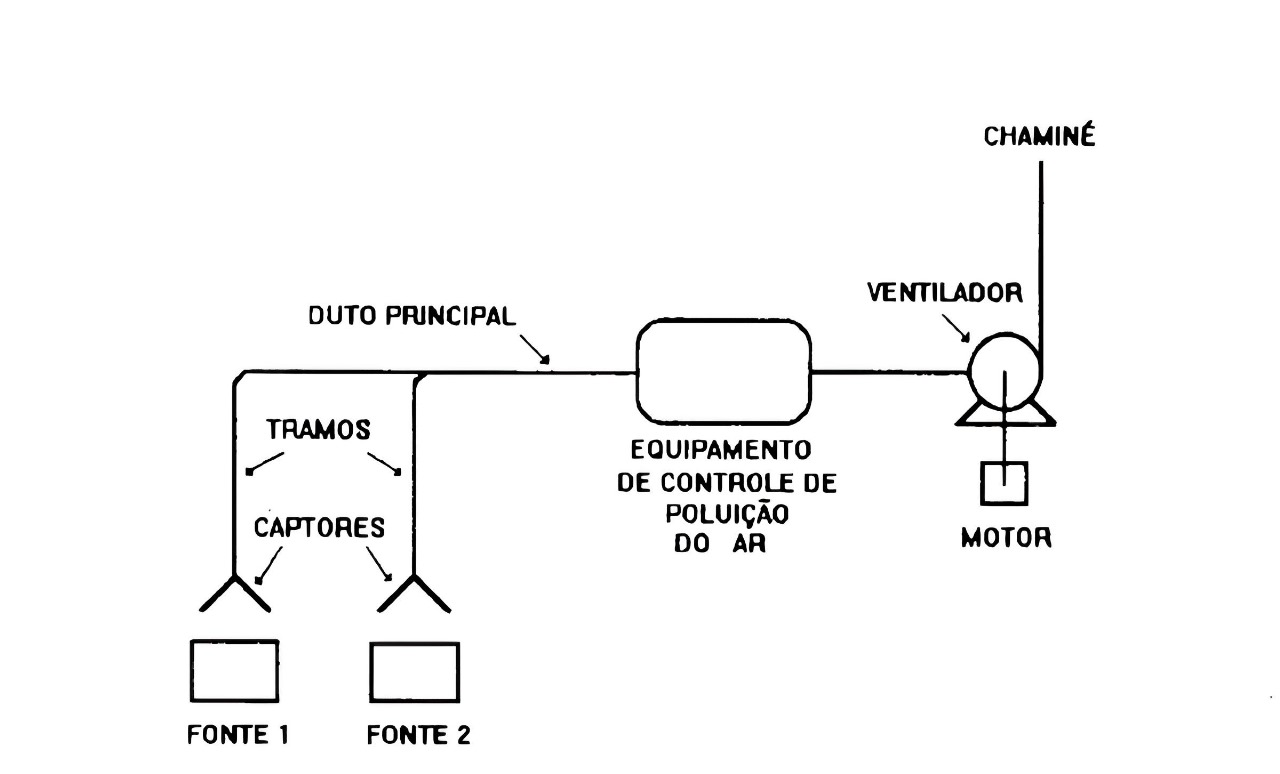
\includegraphics[width=0.7\linewidth]{Imagens/VLE.jpeg}
    \smallcaption{Fonte: \textcite{livrocetesb}}
    \label{fig: compnentes da VLE}
 \end{figure}

Um fator importante a ser destacado no dimensionamento por VLE é a obtenção das velocidades de captura e da distância de partícula ao longe, à face do captor. As velocidades de do sistema estão esquematizadas na Figura \ref{fig: velocidade de captura}.

 \begin{figure}[!htb] 
 \centering
    \caption{\centering Velocidade de Captura}
    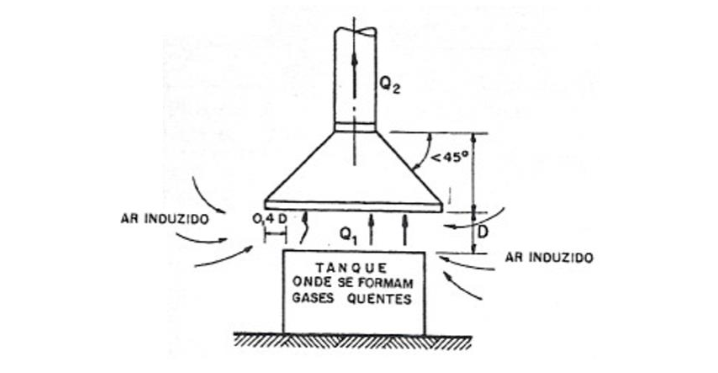
\includegraphics[width=0.8\linewidth]{Imagens/velocidade captura.png}
    \smallcaption{Fonte: \textcite{ventilacaoindustrial}}
    \label{fig: velocidade de captura}
 \end{figure}



\section{Dinâmica dos Fluidos Computacional (CFD)}

Fluxos e fenômenos relacionados podem ser descritos a partir de equações parciais diferenciais, as quais, usualmente, não podem ser resolvidas analiticamente. Dessa maneira, o método da discretização permite aproximar tais equações a um sistema algébrico que possa ser solucionado por meios computacionais. Assim, as aproximações são aplicadas a pequenos domínios de espaço e tempo \cite{peric2002computational} para simular o fenômeno em um determinado período e, portanto, quanto menor a malha utilizada, isto é, quanto menor o domínio de espaço e tempo adotado, maior a precisão dos resultados, embora exija maior capacidade computacional. Assim, a análise numérica dos escoamentos é denominada Dinâmica dos Fluidos Computacional que, em inglês, é representada pela sigla $CFD$. 

Em estudos de conforto térmico a dinâmica dos fluidos computacional é muito utilizada por ser uma ferramenta que consegue simular de maneira muito exata as condições térmicas do ambiente.   

Como um exemplo de estudo de conforto térmico por $CFD$ é possível citar o estudo realizado por \textcite{li2019multi}. Este artigo tinha como objetivo estudar o conforto térmico dentro do carro de um trem de alta velocidade ($HST$) chinês, por meio de simulações $CFD$ e posteriormente utilizar a krigagem (ou $Kriging$, em inglês), para substituir a simulação por dinâmica dos fluidos computacional, por ser mais rápida e otimizada. 
Para chegar em resultados confiáveis e com o mínimo de erros computacionais possíveis, foram feitas 25 simulações, no $software$, com parâmetros diferentes mas com as mesmas resoluções de malha e condições de contorno. Com os resultados das simulações, foi possível obter parâmetros como temperatura da cabine do carro, concentração de contaminantes e o $PMV$ ($Predicted$ $mean$ $vote$) que é um modelo desenvolvido por \textcite{fanger1970thermal}, muito utilizado em estudos de conforto térmico, no qual se utiliza a temperatura da pele para definir o conforto.


\chapter{Materiais e Métodos}

\section{Metodologia}

O objeto deste estudo é um dos carros da frota J da linha 1 - Azul, do Metrô de São Paulo. Esta frota é uma modernização da antiga frota A, de 1974, e foi inaugurada em 2011, sendo sua última modernização em 2018. Um carro desta frota e o mapa da rede do metrô e trem de São Paulo são mostrados nas Figuras \ref{fig:Trem_da_Frota_J_J46} e \ref{fig:mapa-da-rede-metro-0124-abre}. Por motivos de sigilo e segurança, os tamanhos reais e as plantas do metrô não poderão ser mostradas, nem divulgadas.

\begin{figure}[!htp]
\begin{subfigure}{0.5\textwidth}
    \caption{Trem da frota J do Metrô de São Paulo}
    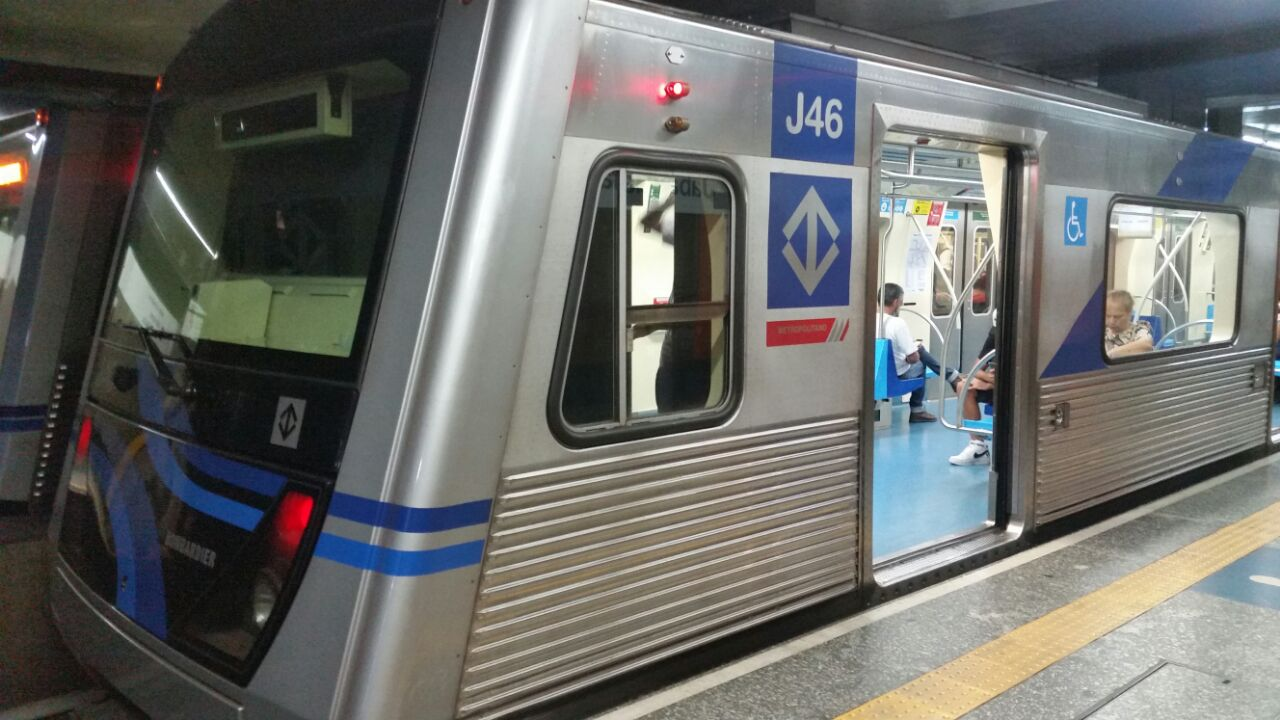
\includegraphics[width=0.9\linewidth, height=6cm]{Imagens/Trem_da_Frota_J_J46} 
    \smallcaption{Fonte: \textcite{frotaJ}}
    \label{fig:Trem_da_Frota_J_J46}
\end{subfigure}
\begin{subfigure}{0.5\textwidth}
    \caption{Mapa da rede de trem e metrô da cidade de São Paulo}
    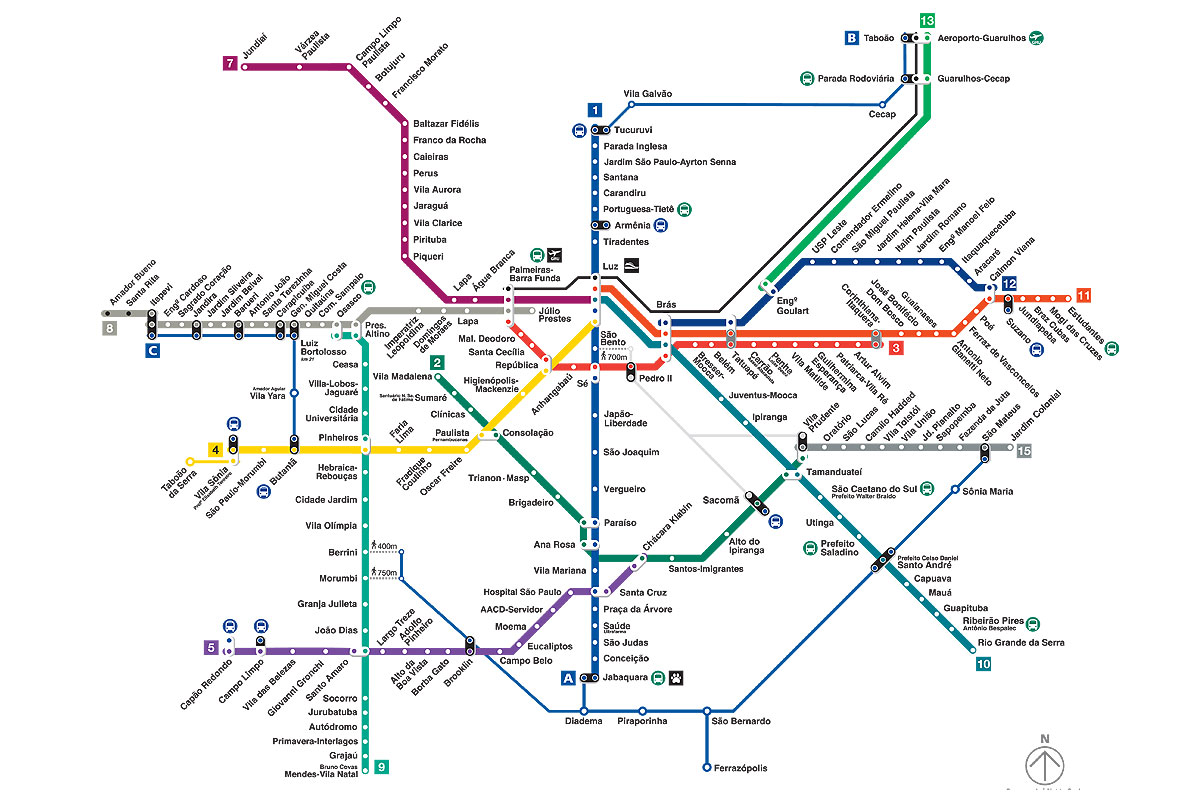
\includegraphics[width=0.9\linewidth, height=6cm]{Imagens/mapa-da-rede-metro-0124-abre.jpg}
    \smallcaption{Fonte: \textcite{Mapametro}}
    \label{fig:mapa-da-rede-metro-0124-abre}
\end{subfigure}
\end{figure}


Será feita a pesquisa da análise dos parâmetros de conforto térmico, levando em conta a ideia e o conceito de VGD (ventilação geral diluidora). Após a conclusão da pesquisa e das revisões bibliográficas, serão realizadas reuniões pontuais com a equipe do Metrô São Paulo, nas quais as ideias do grupo serão alinhadas e discutidas com a empresa. 

A seguir, será feita a escolha dos melhores sensores considerando o custo benefício e aplicação específica empregada. Para validar o funcionamento de todos os sensores e o código desenvolvido, serão realizados testes iniciais utilizando uma $protoboard$, garantido assim o funcionamento de tudo em conjunto, podendo-se assim seguir para próxima parte que será o desenvolvimento de três placas de circuito impresso (PCB), com todos os componentes já integrados. 

Duas placas serão iguais, e têm o intuito de permanecer dentro do vagão do Metrô, realizando a medição das informações em dois locais estratégicos, sendo estes a tubulação de insuflamento e de retorno do carro. A partir de uma conversa com o Metrô, foi sugerido o posicionamento tanto em armários internos ao carro, como nas próprias tubulações, sendo a segunda opção a escolhida, como mencionado. Com isso, é possível ter uma noção de o que é colocado no ambiente, e do que é retirado do mesmo. A terceira placa, por sua vez, será posicionada em um local externo ao recinto dos passageiros, para que seja possível realizar uma comparação entre os dois. É válido citar que o posicionamento destas placas depende da autorização do Metrô, visto que não podem interferir com o funcionamento para o usuário.
 

Em seguida, a partir das PCBs e o código de obtenção dos dados validados, ocorrerá a instrumentação do carro do metrô com base nas plantas elétricas e de ventilação disponibilizadas. Com a finalização desse processo, o sistema de aquisição de dados realizará a coleta por um período de tempo determinado, possibilitado uma quantidade significativamente grande de dados para serem tratados e analisados futuramente.

Sucessivamente, com posse dos dados obtidos pelos sensores e os disponibilizados pelo Metrô São Paulo, será realizado o tratamento desses dados em um software dedicado e serão elaboradas as primeiras análises do comportamento que o ar possui no carro, e criação de correlações.

Posteriormente, utilizando o que há de mais moderno, a análise computacional a partir do $CFD$, serão gerados novos dados complementares aos instrumentais, levando como base as plantas de ventilação disponibilizados pelo Metrô São Paulo.

Ao final, a comparação dos dados obtidos pela instrumentação com os dados da análise do $CFD$, dará a robustez suficiente para uma conclusão objetiva do que o Metrô São Paulo está fazendo ou do que poderia melhorar. 

\section{Premissas do Projeto}

\subsection{Conjunto de normas}

%ISO 19659-2:202

%-NR17: estabelece temperatura de conforto para escritórios (não sei se usaremos)
%-NR15: normas de insalubridade, saúde e segurança, estresse de temperatura, radiação 
%-Carta bioclimatica do Brasil: sensação de conforto termico é obtida para umidade relativa variando de 20 a 80\% e temperatura entre 18 e 29 graus celsius; possibilita propor soluções para alcançar o conforto termico
%-industrial ventilation: guia de recomendações para ventilação de ar

\section{Sistema de aquisição de dados}

A aquisição de dados é parte fundamental do trabalho, sendo a base para futuras análises e correlações. Como descrito na seção \ref{ventilação}, certos parâmetros como temperatura, umidade e a qualidade do ar interferem diretamente na percepção do que é agradável ou não para as pessoas. Logo é necessário uma robustez dos dados que serão coletados e aferidos.

Parte dos dados apresenta carácter quantitativo, como a temperatura do ar de insuflamento e o ar de retorno. Outros dados se apresentam em carácter mais qualitativo, como a opinião das pessoas sobre a temperatura em um determinado estado de tempo, e parte do trabalho é analisar a correlação desses dados.

Além da divisão dos tipos de dados há a divisão da fonte dos mesmos, sendo que uma parte dos dados será obtida diretamente pelo Metrô São Paulo, como:
\begin{itemize}
    \item Reclamação dos usuários;
    \item Peso do carro;
    \item Abertura e Fechamento da porta do carro;
    \item Temperatura.
\end{itemize}    
E uma segunda parte dos dados será obtida a partir da instrumentação adicional do carro:
\begin{itemize}
    \item Temperatura;   
    \item Umidade; 
    \item Pressão Barométrica
    \item Concentração de $CO_2$;  
    \item Concentração de particulados.
\end{itemize}    

Deste modo, é possível definir os três kits que serão montados como os dois Kits Internos, que permanecerão nas tubulações internas, como já mencionado, composto cada um por um microcontrolador acoplado ao PCB com sensores de temperatura, umidade, concentração de $CO_2$ e de particulados, e o Kit Externo, cuja localização ainda depende de um alinhamento de ideias com a equipe do Metrô, composto também por um microcontrolador acoplado ao PCB mas somente com sensores de temperatura, umidade e pressão barométrica. É válido citar também que cada PCB deverá ter um sensor de cada, entretanto conforme o decorrer do projeto, este valor pode ser alterado. 

\subsection{Sensores} \label{sensor}

De modo a obter êxito na conclusão dos objetivos gerais e específicos deste trabalho, é necessária a utilização de alguns sensores propícios à obtenção dos dados quantitativos previamente citados. Um sensor nada mais é do que um equipamento que, em contato com o ambiente que se deseja analisar, transforma variações físicas em um sinal elétrico correspondente, que deve posteriormente ser recebido, interpretado, e armazenado, com o auxílio de um controlador. Assim, estes sensores devem ser capazes de funcionar no local de estudo, um dos carros do metrô de São Paulo, por suficiente tempo para a obtenção das informações necessárias para posterior correlação com os dados qualitativos obtidos da própria instituição estudada. É válido também citar que, durante uma conversa com o Metrô, foi indicada a possibilidade de uso de alguns sensores já instalados no vagão, como o de temperatura, peso e indicador de abertura de portas.

O sensor de temperatura que será utilizado, DS18B20, opera de 3,0 a 5,5 $Volts$ e foi escolhido devido a sua boa reputação em aplicações ligadas a $HVAC$ e facilidade de montagem, ao funcionar com protocolo $One-Wire$, onde, além da pinagem necessária para energização, $GND$ e $VDD$,  padrão para todos os componentes, transmite seus dados aquisitados por apenas uma via, denominada $DQ$, havendo tanto envio quanto recebimento de sinal por meio de uma porta digital.  O $layout$ desta pinagem é apresentado na Figura \ref{fig:PinTemp}, onde são vistos, além dos pinos citados, as letras "NC", que dizem respeito à conexões não utilizadas.

\begin{figure}[!htb]
\centering
    \caption{Diagrama da pinagem do sensor DS18B20}
    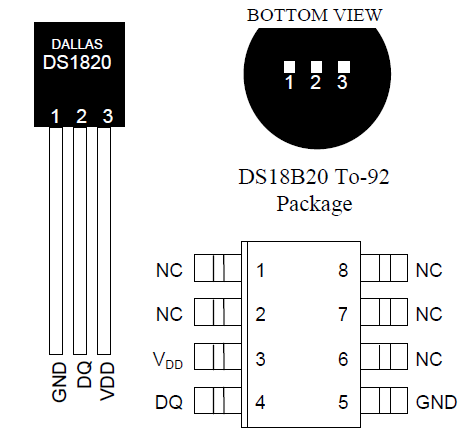
\includegraphics[width=0.6\linewidth]{Imagens/PinTemp.png}
    \smallcaption{Fonte: \textcite{DS18B20}.}
    \label{fig:PinTemp}
\end{figure}

Outras vantagens deste sensor incluem sua capacidade de funcionamento sem outros componentes, o que elimina a necessidade de uma placa de interpretação, por exemplo, além de um intervalo de medição de temperatura satisfatório ao projeto, variando entre -55$°C$ a +125$°C$, com uma resolução padrão de 0,5$°C$, configurável até 0,0625$°C$ a partir de uma alteração do número de $bits$ utilizados para leitura. 

De acordo com seu $datasheet$, de onde foram extraídos os dados supramencionados, este equipamento opera, de maneira simplificada, com base em uma variação de tensão produzida conforme alteração da temperatura, que por sua vez é convertida como um sinal digital e armazenada na memória interna do dispositivo, composta por 16 $bits$ e denominada de $scratchpad$. Este valor é enviado ao controlador, que recebe e armazena os dados coletados. O diagrama de blocos referente ao sensor pode ser visto na Figura \ref{fig:DiagBlocTemp} 

\begin{figure}[!htb]
\centering
    \caption{Diagrama de blocos para o sensor DS18B20}
    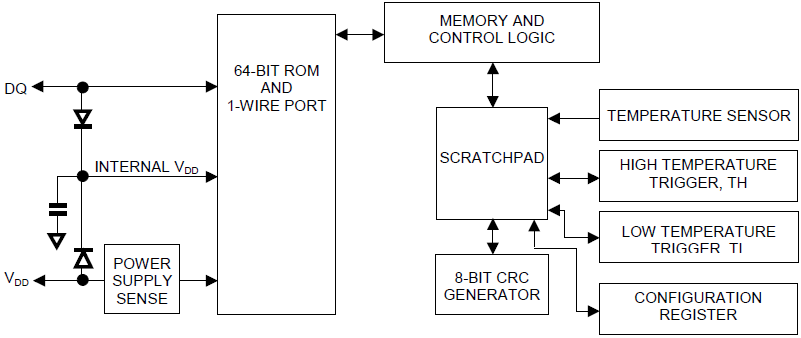
\includegraphics[width=0.8\linewidth]{Imagens/DiagBlocTemp.png}
    \smallcaption{Fonte: \textcite{DS18B20}.}
    \label{fig:DiagBlocTemp}
\end{figure}

Além das vantagens já mencionadas, outro benefício deste equipamento relevante ao trabalho desempenhado diz respeito à sua função de alarme, que funciona a partir dos gatilhos presentes "$HIGH$ $TEMPERATURE$ $TRIGGER$, $TH$" e "$LOW$ $TEMPERATURE$ $TRIGGER$, $TL$", vistos também na Figura \ref{fig:DiagBlocTemp}, para altas e baixas temperaturas, respectivamente. Contanto que a função tenha sido especificada no código que roda no controlador, um conjunto de sensores DS18B20 em paralelo pode perceber uma variação acima dos limites definidos pelo usuário e acusar qual sensor recebeu esta informação, indicando, por exemplo, uma discrepância maior de temperatura na região próxima à abertura das portas do carro. Existem diversas bibliotecas para o uso desse sensor, como a $Arduino$ $Temperature$ $Control$ $Library$ do \textcite{Arduino-Temperature-Control-Library}.

A respeito do sensor de umidade selecionado, HDC1080, seu $datasheet$ revela que opera em um intervalo de voltagem similar ao de temperatura, de 2,7 a 5,5 $Volts$, além de possuir uma precisão satisfatória quanto à obtenção de valores de umidade relativa, variando em apenas 2\%, validando a coleta de dados. Outras vantagens incluem o baixo consumo energético e pequeno tamanho, o que facilita a montagem no espaço à ser utilizado dentro do vagão. A pinagem necessária pode ser vista na Figura \ref{fig:PinHum}, onde $SDA$ representa a linha serial de dados, que deve ser conectada ao controlador, transmitindo em velocidade padrão de 11 $bits$ por segundo, $SCL$ representa o relógio serial, que mantém o conjunto controlador/sensor em sincronia, e $GND$, $VDD$, e "NC" cumprem as mesmas funções previamente citadas.

\begin{figure}[!htb]
\centering
    \caption{Diagrama da pinagem do sensor HDC1080}
    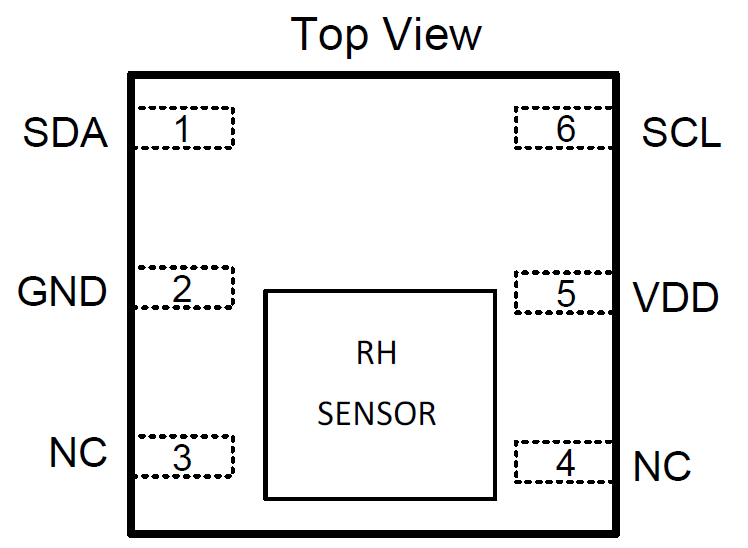
\includegraphics[width=0.6\linewidth]{Imagens/PinHum.png}
    \smallcaption{Fonte: \textcite{HDC1080}.}
    \label{fig:PinHum}
\end{figure}

Existem outros motivos que levaram a escolha deste sensor, dentre eles a ótima reputação de sua fabricante, $Texas$ $Instruments$, que sugere dentro do próprio $datasheet$ a aplicação em sistemas de $HVAC$, condizendo com o caso estudado pelo grupo, mas também a presença de um sensor secundário de temperatura. Este sensor será de grande auxílio às análises, pois apresentará um carácter de validação ao trabalhar em conjunto com os sensores de temperatura já utilizados, tanto do metrô, quanto o escolhido pelo grupo. A partir de um conjunto de sensores com a mesma função, é possível confirmar que os dados colhidos condizem com a realidade, descobrir padrões, ou ainda encontrar um aparelho defeituoso, por exemplo. 

Assim, é de interesse do grupo utilizar este sensor suplementar, que opera de modo muito similar ao sensor de temperatura previamente mencionado, em conjunto com a leitura da umidade, que ocorre com a reação entre a camada de poliamida do sensor e a umidade do ar, que é traduzida para um valor de resistência, e pode por sua vez ser interpretada como um sinal digital no controlador. Um diagrama de blocos que representa a operação pode ser visto na Figura \ref{fig:DiagBlocHum}, onde "MCU" representa o controlador.

\begin{figure}[!htb]
\centering
    \caption{Diagrama de blocos para o sensor HDC1080}
    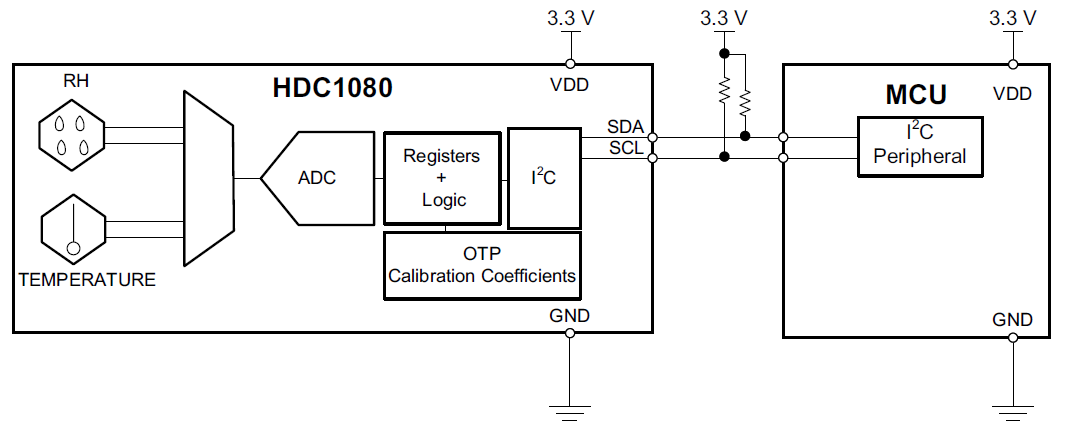
\includegraphics[width=0.8\linewidth]{Imagens/DiagBlocHum.png}
    \smallcaption{Fonte: \textcite{HDC1080}.}
    \label{fig:DiagBlocHum}
\end{figure}

Outras vantagens deste sensor incluem a funcionalidade $HEAT$, que aquece o sensor de modo à reduzir a condensação que pode se acumular no próprio, derivada especialmente de uma operação próxima à um sistema de ar condicionado, além de seu próprio modo de funcionamento, que se divide em um modo de operação, onde o sensor aquisita e envia seus dados, e um modo dormente, onde permanece aguardando uma nova coleta e consumindo quantidades negligenciáveis de energia. A biblioteca existente para esse sensor é a $ClosedCube$ HDC1080 $Arduino$ do \textcite{ClosedCubeHDC1080}.

Sobre o sensor de $CO_2$, o modelo escolhido foi o SCD30, produzido pela $SENSIRION$. De acordo com seu $datasheet$, sua voltagem de operação varia de 3,3 a 5,5 $Volts$, sendo capaz de realizar medições dentro do intervalo de 400 a 10000 $partes$ $por$ $milhão$ para uma variação de apenas 30 $ppm$. Este modelo já vem calibrado de fábrica, o que também facilita o trabalho do grupo frente as análises que devem ser realizadas. O consumo de corrente médio é de 19 $mA$, chegando à um máximo de 75 $mA$ durante as medições, além de operar em temperaturas de 0 a 50 $°C$, o que é satisfatório para o projeto. 

Um diagrama indicando a pinagem do sensor pode ser visto na Figura \ref{fig:PinCO2}, onde $VDD$ e $GND$ cumprem as mesmas funções já mencionadas, $TX/SCL$ faz a transferência de dados do sensor para o controlador, além do relógio serial, $RX/SDA$ recebe informações vindas do controlador, como um pedido de início de medição, por exemplo, $RDY$ indica que os dados estão prontos para coleta, $PWM$ envia um valor de voltagem variável que indica a concentração de $CO_2$ e $SEL$ seleciona as diferentes interfaces do sensor.

\begin{figure}[!htb]
\centering
    \caption{Diagrama da pinagem do sensor SCD30}
    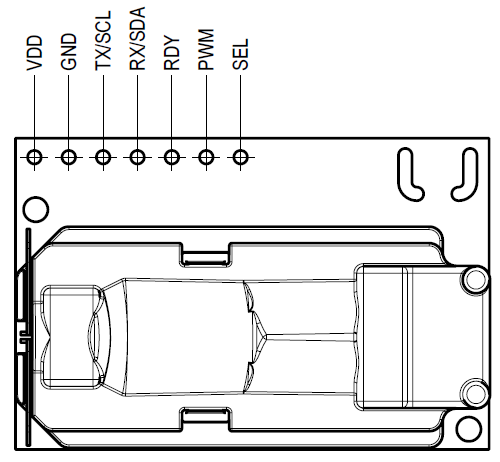
\includegraphics[width=0.6\linewidth]{Imagens/PinCO2.png}
    \smallcaption{Fonte: \textcite{SCD30}.}
    \label{fig:PinCO2}
\end{figure}

Este dispositivo utiliza a tecnologia $NDIR$ , ou $Nondispersive$ $infrared$, para realizar a leitura dos níveis de $CO_2$ no ambiente. De maneira simplificada, o sensor utiliza um pequeno diodo emissor de luz infravermelha instalado dentro de um tubo que se comunica com o ambiente via uma entrada e saída.  Neste invólucro, há também um sensor óptico baseado nas características de uma molécula de $CO_2$,  de modo que quando o ar dentro deste tubo é bombardeado com a luz mencionada, há uma absorção dos raios por parte das moléculas do gás analisado, fazendo com que o sensor óptico, ao realizar a leitura, obtenha uma concentração menor do que a prévia, para um caso de aumento da substância estudada, por exemplo \cite{NDIR}. Esta diferença é, então, contabilizada pelo sensor que, por sua vez, envia os dados para o controlador, e assim a medição é concluída.

É válido citar que, de modo similar ao sensor de umidade escolhido, este sensor de $CO_2$ também possui equipamentos redundantes ao projeto, como um sensor de temperatura e um de umidade relativa, ambos com características satisfatórias ao necessário para a análise. Como já foi citado, estes sensores auxiliares validam as coletas realizadas, garantindo uma maior credibilidade ao estudo. Além disso, a presença deste sensor dispensa a necessidade de outro para aquisição de $O_2$, visto que este parâmetro pode ser estimado a partir dos resultados obtidos. A biblioteca existente para esse sensor é a $Adafruit$ SCD30 do \textcite{Adafruit_SCD30} 

De modo a averiguar melhor as condições do ar ambiente, visando a saúde dos ocupantes do Metrô, foi escolhido também um sensor de particulados suspensos no ar. A partir de um determinado tamanho, as partículas suspensas deixam de ser filtradas pelo sistema respiratório humano, podendo então se acumular nos pulmões ou até mesmo adentrar na corrente sanguínea, causando desde irritação até problemas cardio-respiratórios \cite{pm25}. De 2,5 a 10 $\mu$$m$, as partículas são consideradas grossas, e tem apenas a possibilidade de passar para o pulmão, porém, para substâncias ainda menores, de 0,1 a 2,5 $\mu$$m$, são consideradas finas e entram no corpo com facilidade, sem uma rota de saída definida. Com isso em mente, foi selecionado o sensor PMS5003, um que realiza medições de particulados no ambiente em um intervalo de 0,3 a 10 $\mu$$m$, o que pode indicar a presença de material nocivo no ar.

O modelo selecionado, produzido pela $PLANTOWER$, possui uma eficiência de até 50\% para partículas de 0,3 $\mu$$m$, porém apresenta uma eficiência de de 98\% para materiais a partir de 0,5 $\mu$$m$. Além disso, utiliza também 5 $Volts$ para seu funcionamento, com um consumo de corrente um ligeiramente acima dos outros sensores, podendo chegar até 100 $mA$, mas trabalha em intervalos de temperatura e umidade satisfatórios ao projeto. Seu pequeno tamanho e proteção embutidas também influenciaram na escolha, pois garantem que o sensor pode ser facilmente colocado no vagão e sofrerá de baixas interferências com alterações no ambiente estudado.

Para a conexão deste sensor ao controlador, pode se apresentar a Figura \ref{fig:PinPart}, retirada do $datasheet$ do aparelho, de onde foram também extraídas as informações mencionadas anteriormente. Os pinos são numerados da direita para a esquerda, sendo o $PIN$ $1$ a conexão $VCC$, $PIN$ $2$ a conexão $GND$, já apresentadas nos outros sensores, $PIN$ $3$ a função $SET$, que determina a condição ativa ou dormente do aparelho, $PIN$ $4$ a porta $RX$, que recebe dados do controlador, $PIN$ $5$ a porta $TX$, que faz o oposto, enviando os dados coletados ao controlador, $PIN$ $6$ a funcionalidade $RESET$, que reinicia a operação, e os $PINs$ $7$ e $8$ pinos inutilizados, caracterizados portanto como "NC". 

\begin{figure}[!htb]
\centering
    \caption{Definição de pinos do PMS5003}
    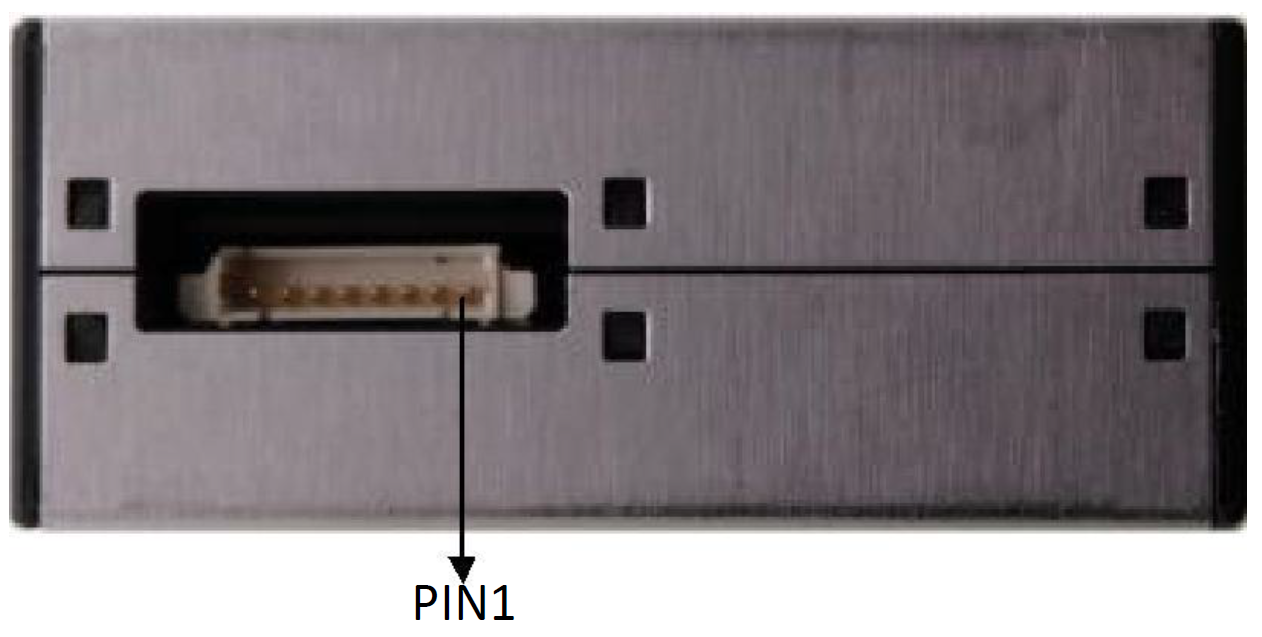
\includegraphics[width=0.6\linewidth]{Imagens/PinPart.png}
    \smallcaption{Fonte: \textcite{PMS5003}.}
    \label{fig:PinPart}
\end{figure}

Torna-se válido também a descrição do princípio de funcionamento deste sensor, que se baseia na dispersão de um $laser$. Dentro do aparelho, há um emissor que produz uma fonte de luz puntiforme posicionada de modo a passar por um canal conectado ao ambiente à se analisar. A partir do "toque" das partículas suspensas nesta cavidade com o $laser$, a luz se espalha, fazendo com que uma superfície capaz de perceber esta dispersão reconheça uma diferença em relação ao momento anterior. Este ciclo se repete durante a medição, que é emitida como um sinal elétrico, que por sua vez é interpretado pelo microprocessador integrado no PMS5003, e finalmente é enviado como um sinal digital ao controlador, indicando o tamanho e quantidade de particulados presentes no ar. Um esquema desta operação pode ser visto na Figura \ref{fig:FuncPart}, sendo esta e as informações retiradas do $datasheet$. A biblioteca existente é a PMS $Library$ de \textcite{ArduinoPMS}.

\begin{figure}[!htb]
\centering
    \caption{Princípio de funcionamento do PMS5003}
    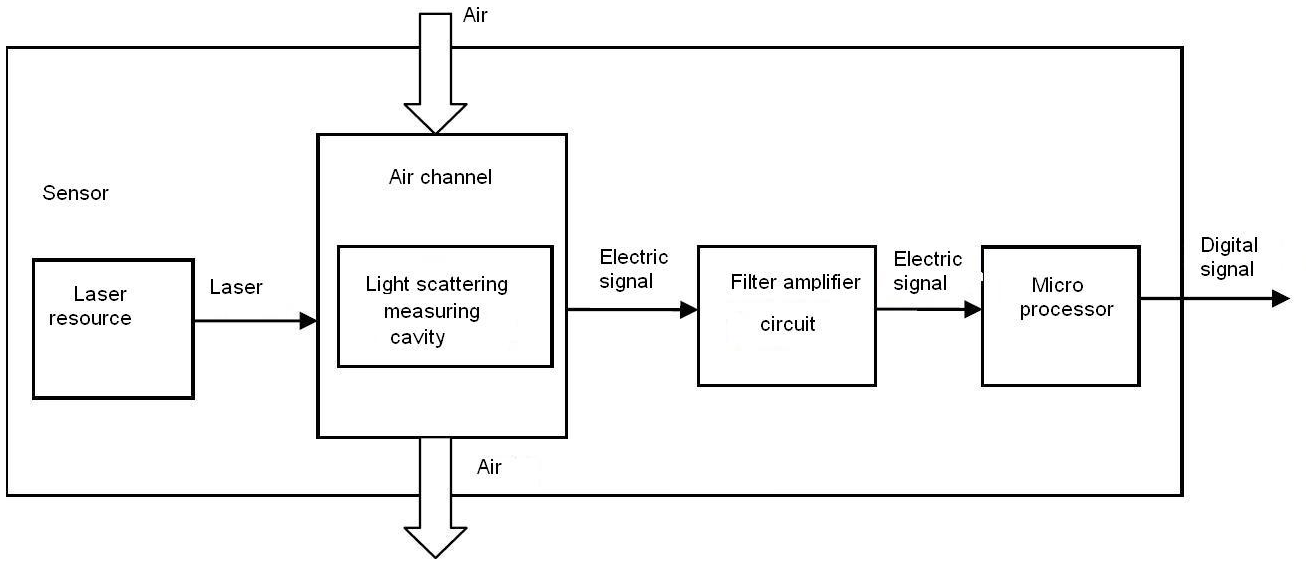
\includegraphics[width=0.8\linewidth]{Imagens/FuncPart.png}
    \smallcaption{Fonte: \textcite{PMS5003}.}
    \label{fig:FuncPart}
\end{figure}

Por fim, a respeito do último sensor selecionado, pode-se citar o BMP280, produzido pela $BOSCH$, 
como o sensor de pressão barométrica escolhido para o projeto. Este sensor realiza a medição da pressão atmosférica absoluta em um intervalo de 300 a 1100 $hPa$, equivalente a aproximadamente +9000 (acima) e -500 (abaixo) metros do nível do mar, com uma precisão de $\pm$ 0,12 $hPa$, equivalente a $\pm$ 1 metro. O sensor realiza estas medições para uma voltagem de 1,7 a 3,3 $Volts$, consumindo uma corrente muito baixa, de 2,7 $\mu$$A$, além de operar dentro de um intervalo de temperatura de -40 a 85 $°C$, condições propícias ao projeto. Entre outras vantagens, há seu pequeno tamanho, visto que foi desenvolvido para aplicações $mobile$, ou seja, para dispositivos móveis, facilitando o posicionamento em local externo ao vagão, já que este sensor é denotado para o kit externo, como mencionado.

A escolha deste sensor foi facilitada, ao considerar além das especificações já mencionadas, a reputação de seu fabricante, que possui anos de experiência nesta e em outras áreas de aplicação. Assim, descrevendo as conexões realizadas com o controlador, tem se a Figura \ref{fig:PinPress}, onde $VCC$ e $GND$ realizam as mesmas funções já citadas, mas para uma conexão de 3,3 $Volts$, $SCL$ representa a entrada do relógio serial, $SDA$ representa a entrada de dados vindos do controlador, $CSB$ representa o seletor de interfaces, já que o sensor pode operar com diferentes controladores (neste caso, deve ser conectado à uma tensão secundária), e $SDO$ realiza o envio dos dados coletados pelo sensor para o controlador. É válido citar que, enquanto estas informações foram extraídas do $datasheet$, este não é o caso da Figura \ref{fig:PinPress}, pois o documento mencionado apresenta diretamente as conexões feitas ao microchip, isto é, diretamente ao sensor, que necessita de uma placa secundária para interface com o controlador selecionado devido ao seu pequeno tamanho.

\begin{figure}[!htb]
\centering
    \caption{Definição de pinos do BMP280}
    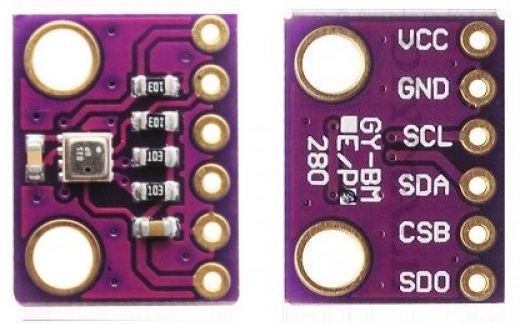
\includegraphics[width=0.8\linewidth]{Imagens/PinPress.png}
    \smallcaption{Fonte: Eletronik LV}
    \label{fig:PinPress}
\end{figure}

A respeito de seu princípio de funcionamento, denominado de piezo resistivo, o mesmo ocorre com a deformação de um diafragma interno por efeito de uma pressão aplicada, geralmente construído de silicone e calibrado com base na pressão a ser medida, neste caso a atmosférica, que é notada por um $strain$ $gauge$, ou seja, um extensômetro, o que causa uma alteração na resistência percebida na ponte de $Wheatstone$ presente dentro do componente. De maneira análoga, conforme a resistência é alterada, a voltagem que passa pelo sensor também sofre uma alteração, o que pode ser enviado para o controlador e interpretado como a pressão atmosférica do ambiente presente \cite{piezo}, sendo um exemplo disto visto na Figura \ref{fig:piezoresist}.

\begin{figure}[!htb]
\centering
    \caption{Princípio de funcionamento de um sensor piezo resistivo}
    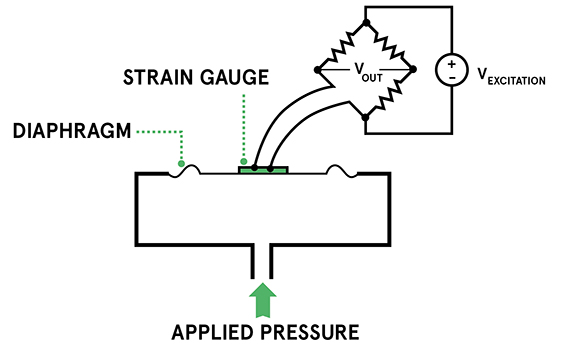
\includegraphics[width=0.8\linewidth]{Imagens/piezoresist.jpg}
    \smallcaption{Fonte: AVNET Abacus}
    \label{fig:piezoresist}
\end{figure}

A partir da medição de pressão barométrica, este sensor permite, portanto, o cálculo da altitude em que se encontra, informação relevante para a obtenção da situação climática, por exemplo. Visto que este sensor está na parte externa do carro, isto é relevante para uma comparação da situação térmica oriunda da previsão/medição do tempo atual no exterior com a do ambiente interno e populado. Além disso, como outra vantagem, este equipamento também possui um sensor de temperatura redundante ao projeto, que será usado com o mesmo propósito de validação de dados. A biblioteca existente para esse sensor é a $Adafruit$ BMP280 do \textcite{Adafruit_BMP280}. 

\subsection{Protoboard}

A partir das escolhas dos sensores na seção \ref{sensor}, conseguiu-se fazer a seleção do microcontrolador. Segundo \textcite{kerschbaumer2013microcontroladores}, os microcontroladores são circuitos integrados que possuem em seu interior todos os componentes necessários para seu funcionamento dependendo unicamente da fonte de alimentação externa. Logo, eles agem como o cérebro de toda a parte eletrônica responsável pelo fluxo de dados e a computação dos mesmos.

A placa de prototipagem escolhida foi o $Arduino$ $Nano$, Figura \ref{fig:pinagem arduino}, integrada pelo microcontrolador $ATmega328$ \cite{UNO}. A principal vantagem da escolha da plataforma $Arduino$, além do seu custo relativamente acessível, é a facilidade para desenvolver software com ela. A linguagem para desenvolver códigos é uma versão simplificada de $C$ e $C++$, e para contribuir ainda mais exitem na casa de milhões de bibliotecas online, que são programas que foram criados por outros usuários que podem ser usadas gratuitamente em outros projetos, facilitando assim boa parte do desenvolvimento do algorítimo base. Os sensores escolhidos já possuem bibliotecas pré-estabelecidas que serão utilizadas pelo grupo.

\begin{figure}[!htb]
\centering
    \caption{Pinagem do Arduino Nano}
    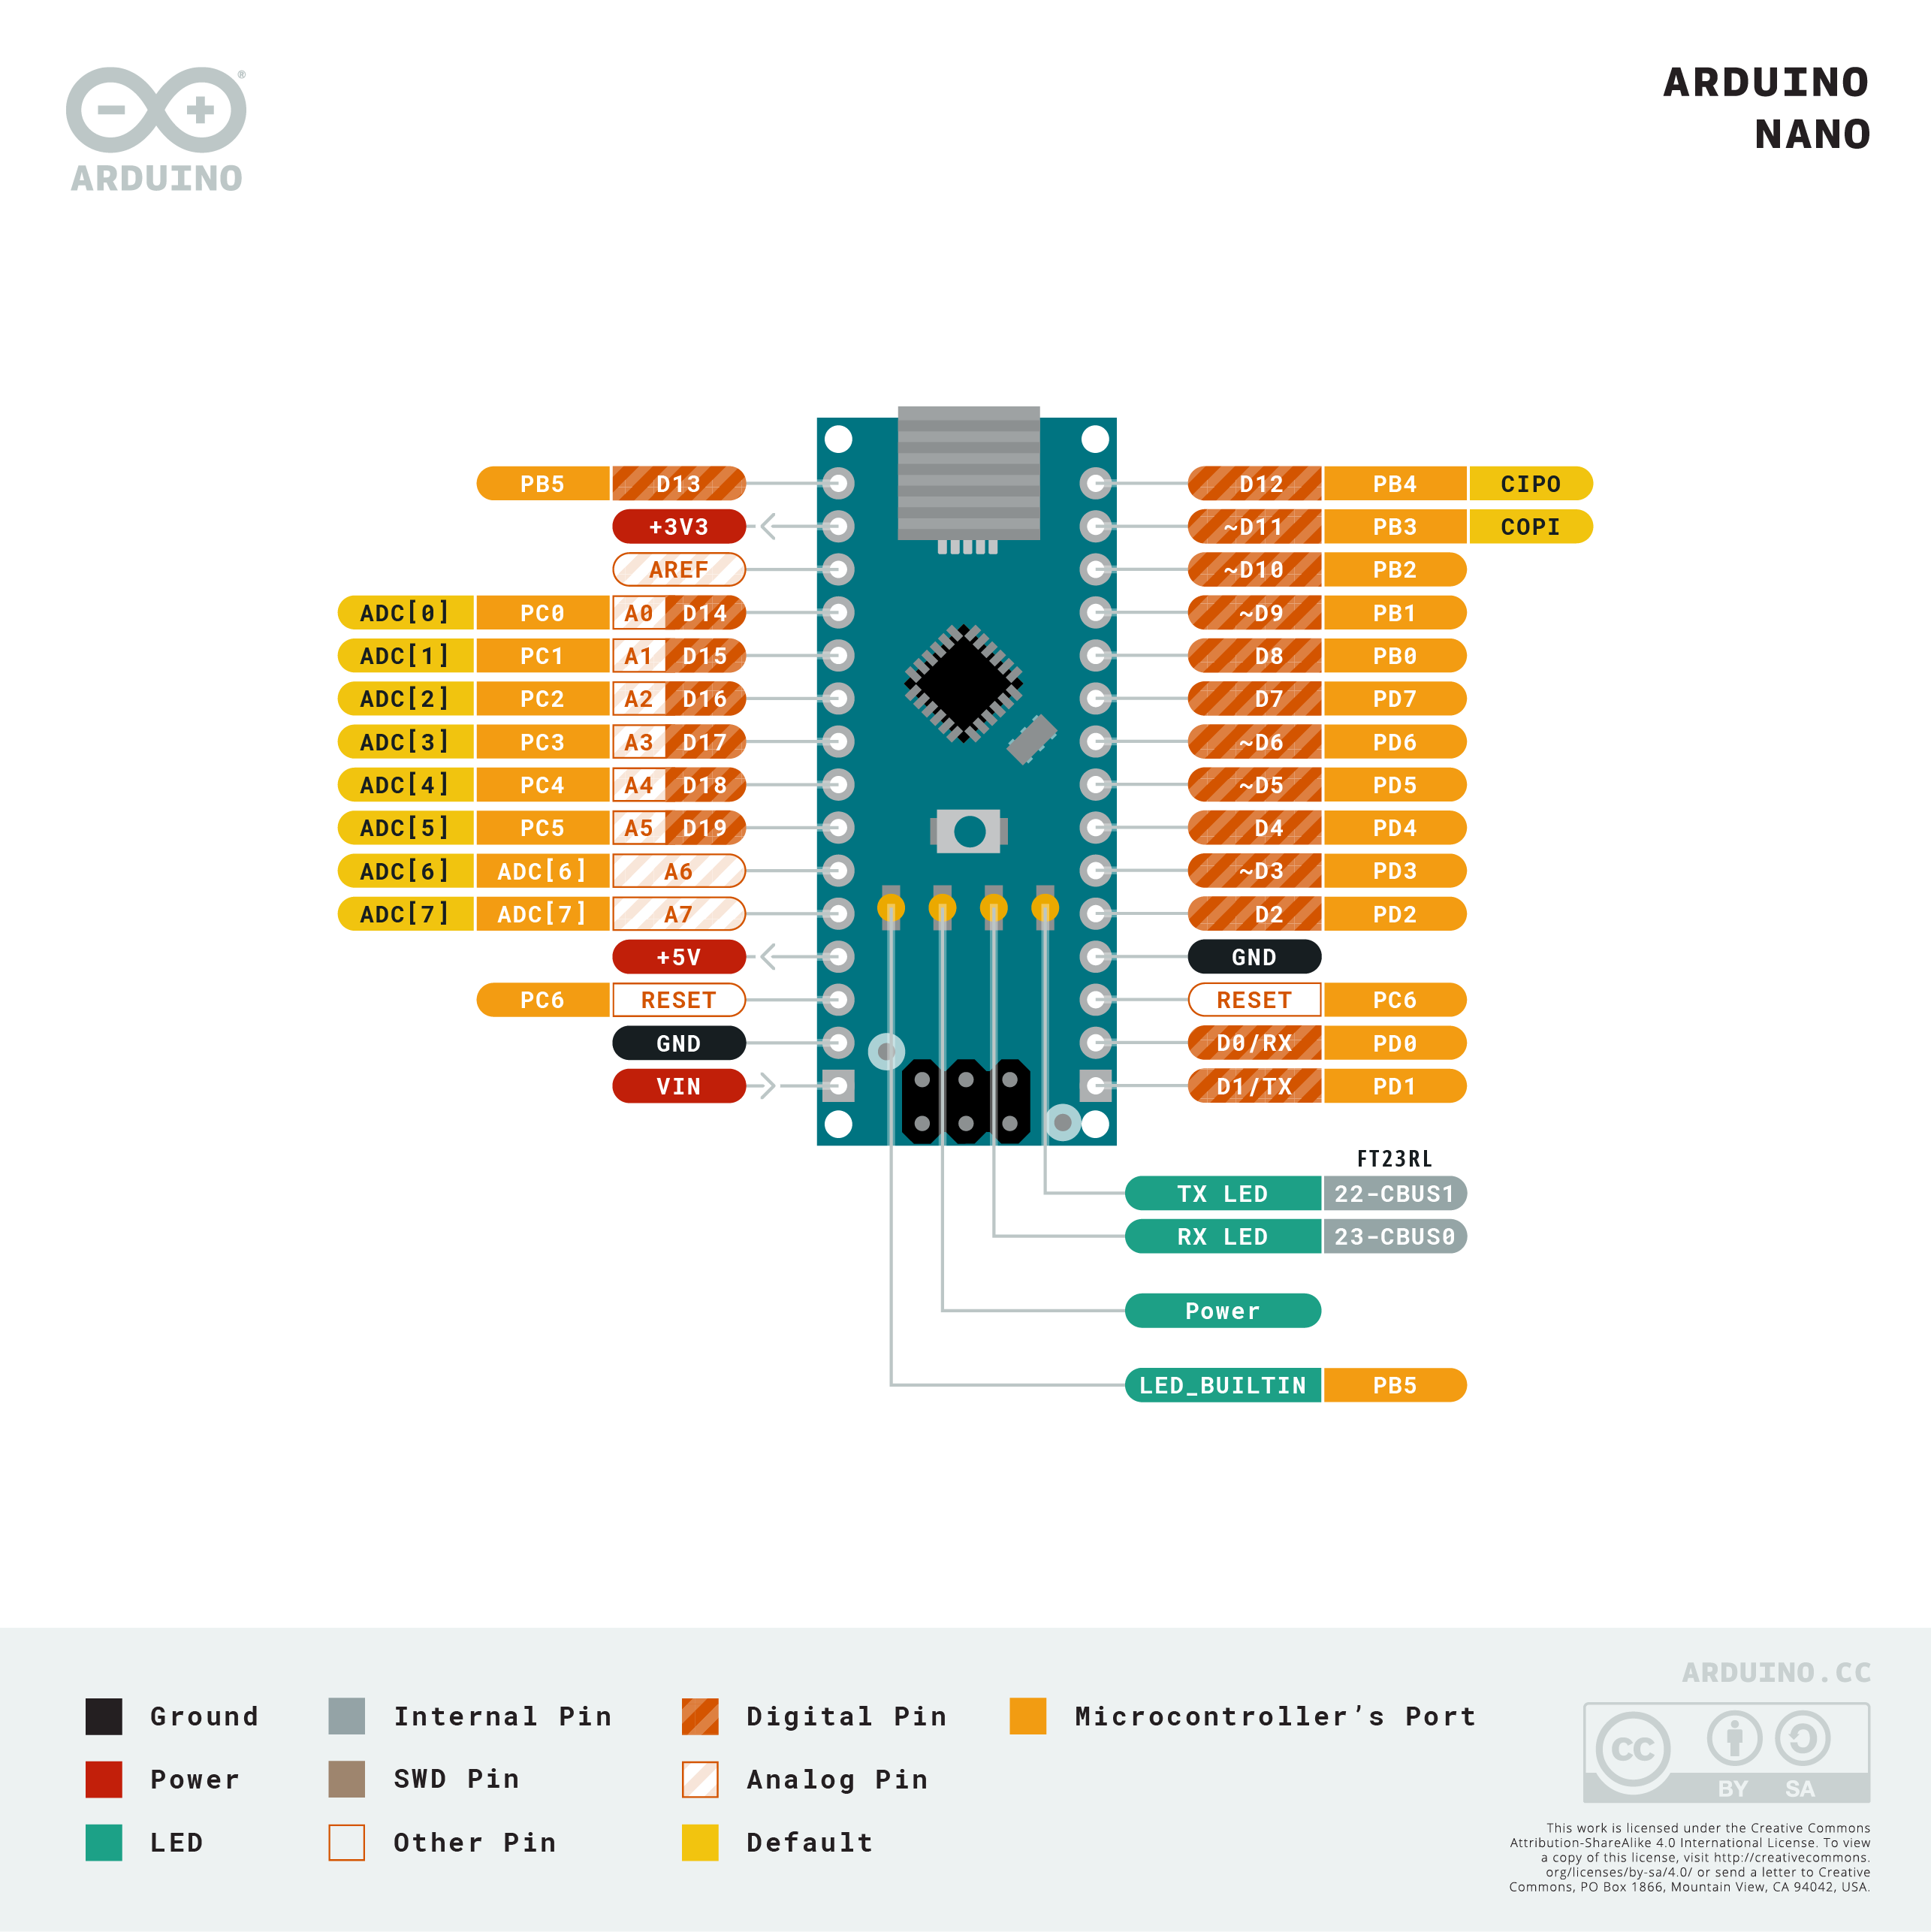
\includegraphics[width=0.85\linewidth]{Imagens/Pinagem Arduino Nano.png}
    \smallcaption{Fonte: \textcite{UNO}}
    \label{fig:pinagem arduino}
\end{figure}

Para armazenamento de dados será utilizado o $MicroSD$ $card$ $breakout$ $board+$ I$D 254$, Figura \ref{fig:FotomicroSD}, que é um adaptador que passa os dados gerados pelos sensores e computorizados pelo $Arduino$ para um cartão $MicroSD$ externo removível, pois o $Arduino$ $Nano$ possui $32kB$ $flash$ de memória \cite{UNO}, o que serve tanto para armazenar o programa feito para ler os sensores, quanto os dados gerados pelo mesmo. Com a utilização do $MicroSD$ $card$ $breakout$ $board+$ é possível transferir todos os dados gerados em um cartão$ MicroSD$ que pode ser de $2GB$ á $2TB$ de memória, resolvendo o problema de armazenamento e conseguindo armazenar o máximo de dados que os sensores conseguirem fornecer. A vantagem de usar um cartão $MicroSD$ para o armazenamento é que já existem bibliotecas para o uso de cartão, sendo uma delas a $FAT16$ $Library$, recomendada pela própria fabricante \textcite{254MicroSD}.

\begin{figure}[!htb]
\centering
    \caption{MicroSD card breakout board+ ID 254}
    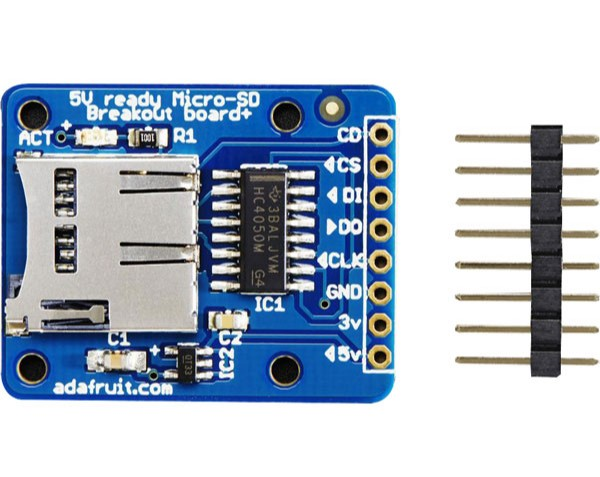
\includegraphics[width=0.45\linewidth]{Imagens/Adafruit 254 Micro SD.jpg}
    \smallcaption{Fonte: \textcite{254MicroSD}}
    \label{fig:FotomicroSD}
\end{figure}

Com a seleção do microcontrolador e do sistema de armazenamento, é possível seguir para o esquemático e montar as $protoboards$, que são as placas de teste que permite a montagem de circuitos eletrônicos temporários, que será usada para testar o funcionamento dos componentes e o código desenvolvido.

Usando como base todos os $datasheet$ dos componentes e o uso do software $KiCAD$ foi possível fazer os primeiros esquemáticos, Figuras \ref{fig:footprintprotoboardint} e \ref{fig:footprintprotoboardext}, que apresenta todos os componentes e conectores escolhidos, e usando uma fonte de 5V, que é a potência que o $Arduino$ $Nano$ e todos os componentes operam. Posteriormente na construção da PCB será necessário incorporar um transformador de potência, pois a bateria do carro pode ser de dois tipo a de 48$V$($\pm30\%$) continua  ou de 72$V$($\pm30\%$) continua.

\begin{figure}[!htb]
\centering
    \caption{Footprint para montar a protoboard - kit de medição interno}
    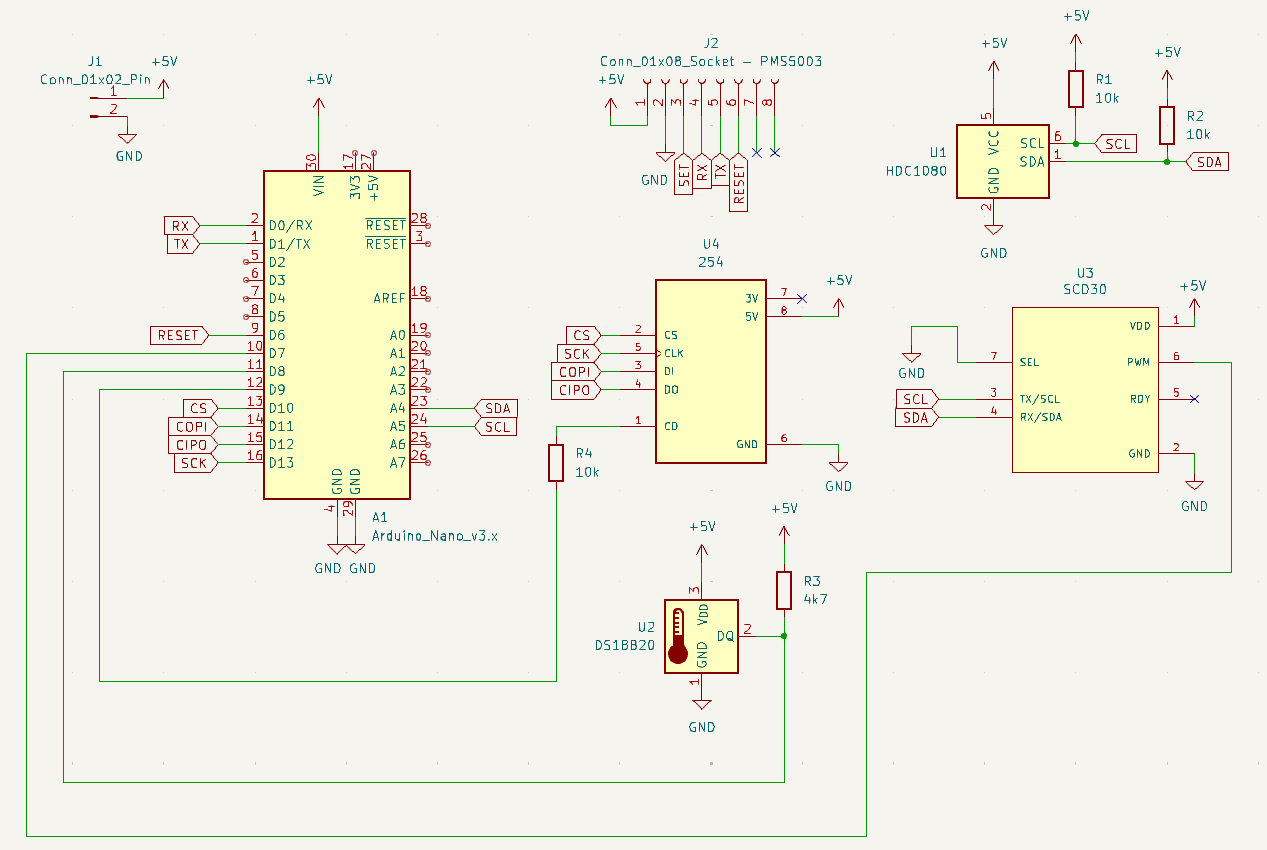
\includegraphics[width=1\linewidth]{Imagens/Footprint protoboard interna.png}
    \smallcaption{Fonte: Autor}
    \label{fig:footprintprotoboardint}
\end{figure}

\begin{figure}[!htb]
\centering
    \caption{Footprint para montar a protoboard - kit de medição externa}
    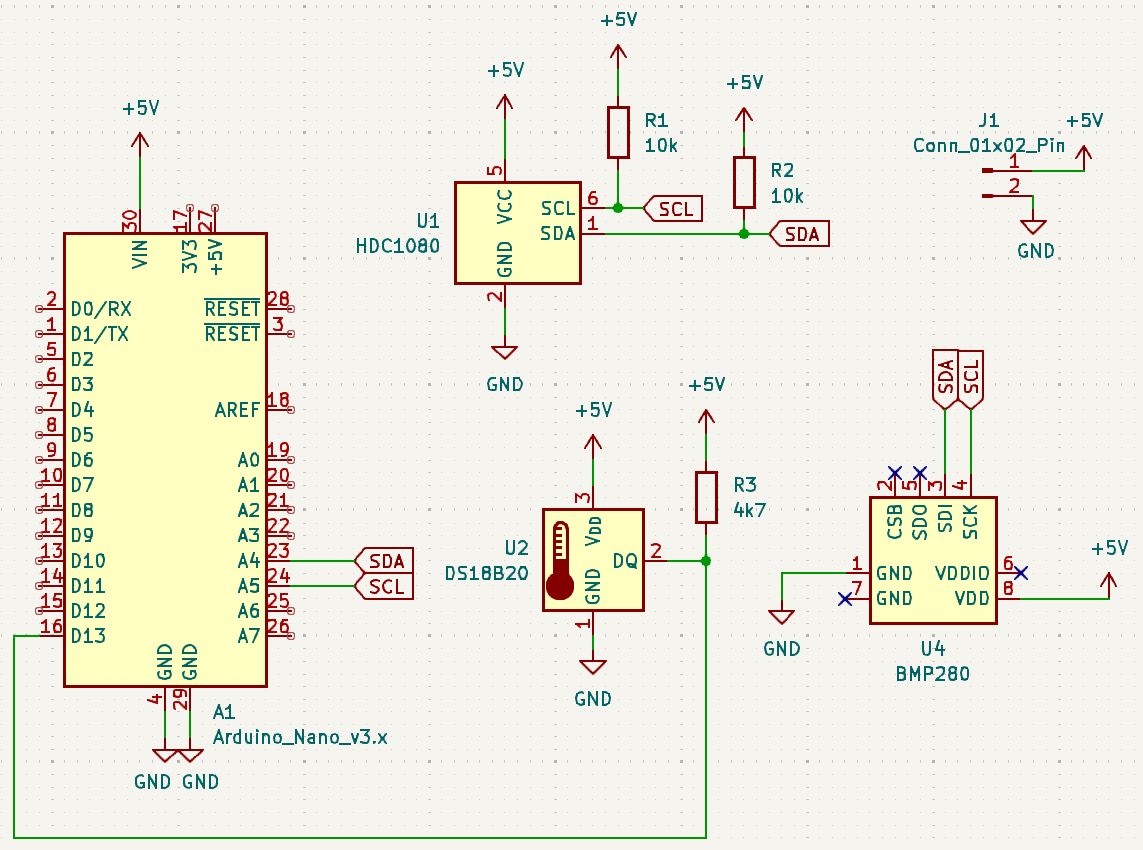
\includegraphics[width=1\linewidth]{Imagens/Footprint protoboard Externo.png}
    \smallcaption{Fonte: Autor}
    \label{fig:footprintprotoboardext}
\end{figure}

\subsection{Placa de Circuito Impresso (PCB) } \label{PCB}

Teste compilador

\section{Instrumentação do carro - Metrô São Paulo}

\section{Sistema de tratamento de dados}

\section{Implementação do CFD}

\chapter{Resultados finais}

\section{Análise dos resultados}

\section{Análise do CFD}

\chapter{Conclusões}

\chapter{Trabalhos Futuros Possíveis}

\printbibliography

\end{document}

